\chapter{Background (SoTA) overview}
\label{chap:sota}

\begin{itemize}
	\item Graph learning intro
		\begin{itemize}
			\item Why graphs?
			\item Tasks
				\begin{itemize}
					\item Node classification
					\item Link prediction
					\item Graph classification
				\end{itemize}
			\item Transductive vs.\ inductive tasks
			\item \cite{gori_new_2005} - overview
		\end{itemize}
	\item Random walk based models
		\begin{itemize}
			\item DeepWalk
			\item LINE?
			\item Node2Vec
		\end{itemize}
	\item MPNNs / convolutional models
		\begin{itemize}
			\item Introduction to message passing
			\item GCN
			\item GraphSAGE
		\end{itemize}
	\item WL test and expressivity in GNNs
		\begin{itemize}
			\item The WL test
			\item The WL test and graph convolution
			\item GIN?
			\item Oversmoothing in graphs
			\item Oversquashing in graphs
			\item The 4 Gs?
		\end{itemize}
	\item Explainability on graphs
		\begin{itemize}
			\item Overview of graph explainability
			\item Instance-level post-hoc explainability
				\begin{itemize}
					\item Gradient-based methods
						\begin{itemize}
							\item Grad-CAM
						\end{itemize}
					\item Surrogate methods
						\begin{itemize}
							\item GraphLime
						\end{itemize}
					\item Perturbation-based methods
						\begin{itemize}
							\item GNNExplainer
							\item PGExplainer
							\item SubgraphX
						\end{itemize}
				\end{itemize}
			\item Model-level explainability
				\begin{itemize}
					\item XGNN
					\item GraphChef?
				\end{itemize}
		\end{itemize}
\end{itemize}


\section{Machine Learning Tasks on Graphs}

\todo{More general intro on graphs before GNNs}
Graphs are a natural way of abstracting many mathematical problems and a versatile data structure used to represent relationships and interactions in various real-world domains such as chemistry, medicine, particle physics, social networks, medicine, fake-news detection, computer network security, autonomous vehicle guidance and others.\todo{Citations} Consequently, machine learning on graphs has, in recent years, seen an explosion in popularity, breadth and depth of both research and applications.

Let us denote a \name{graph} \( G = \left( V, E \right)) \in \mathcal{G} \) where \( V \) is a set of the graph \name{nodes} and \( E \subseteq V^2 \) is a set of \name{edges} connecting the nodes. The questions of whether the edges should be directed, whether to allow self-loops and/or multiple edges between the same pair of nodes is in general not answered. Most of the discussed methods are agnostic to these choices, which are thus left to the user. Optionally, a vector of \name{node features} \( \mathvec{x}_i \in \mathspace{X} \) may be considered for each node \( v_i \in V \). Additionally, these feature vectors are often considered to form a \name{feature matrix} \( \mathmat{X} \in \mathfield{R}^{\left\lvert V \right\rvert \times \left\lvert \mathspace{X} \right\rvert} \) and this feature matrix is then considered to a part of the graph \( G \). \todo{More definitions}

While in traditional machine learning, the range of tasks is usually fairly limited, there are four primary ways of applying machine learning algorithms to graph-structured data; node classification, link prediction, learning over the whole graph and community detection. All four of these tasks share some similarities and various machine learning methods on graphs may be applied to multiple tasks or may be adapted from one task to another. However, this is not a universal property with some methods being specific to one task, or even a particular subclass of that task.

\subsection{Node Classification}

Probably the most common task on graphs is that of \name{node classification}, an example of which can be seen in Figure~\ref{fig:node-classification}. In this scenario, a node label \( y_i \in \mathspace{Y} \) is considered for each node \( v_i \in V \). A subset of training nodes \( V_\mathrm{train} \) is typically used to learn a classification function \( f : \mathcal{G} \times V \to \mathspace{Y} \), that is a function taking a graph and one of its nodes and predicting the label of the given node. This function is then used to predict the class of the remaining nodes, using the information about the graph structure encoded in \( G \) and, optionally, the feature matrix \( \mathmat{X} \). \todo{Applications}

\begin{figure}
	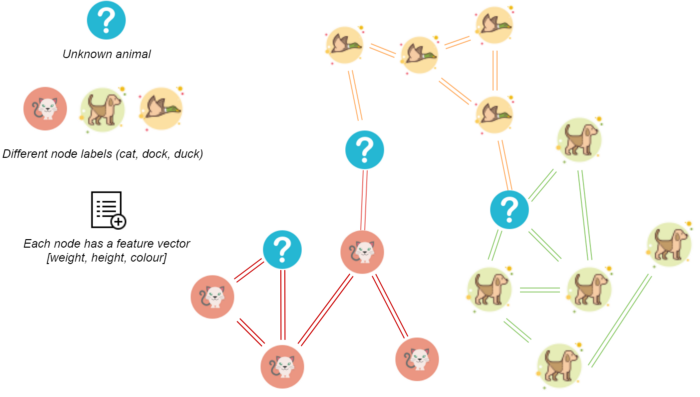
\includegraphics[width=\linewidth]{images/graph-tasks/node-classification.png}
	\caption{A schematic representation of a node classification problem with nodes representing different animals, whose species are the labels of the nodes. Links represent friendships between the different animals. The label is considered to be known for nodes in \( V_\mathrm{train} \) and unknown for other nodes. Original figure from \cite{kubara_machine_2020}.}
	\label{fig:node-classification}
\end{figure}

\subsection{Link Prediction}

The second most common task is that of \name{link prediction}, an example of which is shown in Figure~\ref{fig:link-prediction}. Link prediction focuses on predicting the existence of edges between pairs of nodes in a graph. Given a graph with a set of existing nodes \( E \), the task is to identify potential future or missing edges. This can be framed as a binary classification problem where for each pair of nodes \( (u, v) \in E \), the goal is to predict the probability \( P((u, v) \in E) \). Link prediction is crucial in applications such as recommending friends in social networks, predicting interactions in biological networks, and inferring missing relationships in knowledge graphs.  \todo{References}

\begin{figure}
	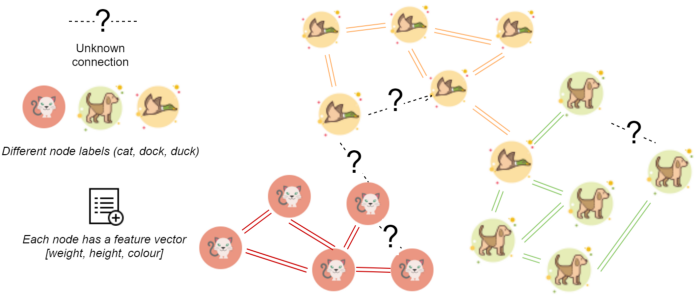
\includegraphics[width=\linewidth]{images/graph-tasks/link-prediction.png}
	\caption{A schematic representation of a link prediction problem with nodes representing different animals, whose species are the labels of the nodes. Links represent friendships between the different animals. Original figure from \cite{kubara_machine_2020}.}
	\label{fig:link-prediction}
\end{figure}

\subsection{Learning over the whole graph}

While node classification and link prediction usually (but not exclusively) concern themselves with tasks within a single graph, it is also possible to consider whole graphs as individual data points. The most common example of this kind of task is \name{graph classification}, where 

Graph classification involves assigning a label to an entire graph rather than individual nodes or edges. Given a set of graphs \( \{G_1, G_2, \ldots, G_N\} \) and corresponding labels \( \{y_1, y_2, \ldots, y_N\} \), the objective is to learn a function \( f: \mathcal{G} \rightarrow \mathcal{Y} \), where \( \mathcal{G} \) denotes the space of all possible graphs and \( \mathcal{Y} \) is the set of labels. This task is common in scenarios where the entire graph structure is indicative of the class, such as in chemical compound classification, where the graph represents the molecular structure, and in document classification, where the graph represents the document's citation or semantic network.

\section{Transductive and inductive learning on graphs}

In the context of machine learning and statistical learning, the terms \name{inductive} and \name{transductive} learning have been used for a long time. In those general fields, the term inductive learning is used for algorithms that use specific training samples to produce general rules, which may then be applied to new samples in the future. In contrast with this stands transductive learning, which foregoes the idea of general rules, instead opting to reason from a set of training samples directly to another set of test samples (see \cite{vapnik_nature_1995}). In the context of graph learning, these two terms are used in a more specific and somewhat different fashion.


\subsection{Inductive Graph Learning}

Inductive graph learning refers to the scenario where the algorithm is trained on a subset of the data and is later evaluated on unseen data. Specifically, the algorithm receives a training set that consists of nodes, edges, labels, and optionally features, and learns a model based on this information. After training, the model is tested on a separate set of data that contains entirely independent nodes, edges, and possibly features, which were not seen during the training phase. When training and test sets are drawn from the same graph, this process is typically achieved by removing the test set from the graph before training. This allows the model to generalize from the training set to new, unseen parts of the graph.

\begin{example}\textbf{Inductive node classification}
	Given a graph \( G = \left( V, E \right) \) with a set of nodes \( V \) and edges \( E \), let \( V_\mathrm{train} \subseteq V \) be the training nodes with known labels, and \( V_\mathrm{test} = V \setminus V_\mathrm{train} \) be the test nodes with unknown labels. The goal in inductive graph learning is to learn the node classification function \( f: \mathcal{G} \rightarrow \mathcal{Y} \) using only \( G \left[ V_\mathrm{train} \right] \), the subgraph of \( G \) induced by \( V_\mathrm{train} \), and \( \mathcal{Y}_\mathrm{train} \), the training node labels. The learned function \( f \) is then evaluated on \( V_\mathrm{test} \).
\end{example}

Inductive methods are more flexible and can handle dynamic and evolving graph structures, making them suitable for applications where the test set is expected to differ from the training set. They are essential for tasks like link prediction in evolving networks or node classification in dynamic environments.

\subsection{Transductive Graph Learning}

Transductive graph learning differs from inductive graph learning in that the algorithm has access to the entire graph, including all nodes, edges, and optionally features, during the training phase. However, the labels for a subset of nodes or edges, referred to as the test set, are withheld. This setting is common in tasks such as node classification and link prediction, where the goal is to infer the missing labels based on the observed graph structure. In transductive learning, the entire graph structure is available during training, but the model only needs to predict the missing labels for the test nodes or edges.

\begin{example}\textbf{Transductive node classification}
	Given a graph \( G = \left( V, E \right) \) where \( V \) is the set of nodes and \( E \) is the set of edges, let \( \mathcal{Y}_\mathrm{train} \) be the labels of the training subset \( V_\mathrm{train} \subseteq V \), and let \( V_\mathrm{test} = V \setminus V_\mathrm{train} \) be the test set of nodes with labels unknown during training. In transductive graph learning, the algorithm aims to learn the node classification function \( f: \mathcal{G} \rightarrow \mathcal{Y} \) that assigns labels to all nodes, utilizing the entire graph structure \( G = \left( V, E \right) \) and the known labels \( \mathcal{Y}_\mathrm{train} \) of the training nodes \( V_\mathrm{train} \). The function \( f \) is then used to predict the labels for the test nodes \( V_\mathrm{test} \).
\end{example}

Transductive methods typically perform well when the test set is not significantly different from the training set, as they can exploit global graph properties and dependencies. However, they usually do not generalize well to new, unseen graphs or nodes.

\section{The graph neural network}

The original \name{Graph Neural Network} (GNN) was first introduced by \cite{gori_new_2005}. While major interest in machine learning on graphs only materialised 10 years later, it is nonetheless this paper that lays the ground work for the entire field. The paper presents a new neural network model called Graph Neural Networks (GNNs), designed to directly process graphs. GNNs extend recurrent neural networks (RNNs) to handle both graph-focused and node-focused applications. The method is based on associating a hidden state vector \( \mathvec{h}_i \in \mathfield{R}^k \) with each node \( v_i \) in the graph, which is updated dynamically according to the node's neighborhood. The update is governed by a parametric transition function \( f_\theta \), which considers the node's label and the states and labels of its neighbors.

Formally, for a graph \( G = (V, E) \), the state \( \mathvec{h}_i \) is defined as the solution to the following system of equations:
\begin{equation}\label{eq:gori-state}
	\mathvec{h}_i = f_\theta \left( y_i, \mathvec{h}_{\mathrm{ne}[v_i]}, y_{\mathrm{ne}[v_i]} \right) , \quad v_i \in V
\end{equation}
where \( y_i \) is the label of node \( v_i \), and \( \mathvec{h}_{\mathrm{ne}[v_i]} \), \( y_{\mathrm{ne}[v_i]} \) represent the states and labels of the neighbouring nodes of \( v_i \), respectively. An output vector \( \mathvec{o}_i \in \mathfield{R}^d \) for each node \( v_i \) is defined using a parametric output function \( g_\theta \):
\begin{equation}\label{eq:gori-output}
	\mathvec{o}_i = g_\theta \left( \mathvec{h}_i, y_i \right) , \quad v_i \in V
\end{equation}

Considering for the whole graph a hidden state matrix \( \mathmat{H} \) and a label vector \( \mathvec{y} \), Equations~\ref{eq:gori-state} and~\ref{eq:gori-output} may be rewritten in a stacked form as
\begin{equation}\label{eq:gori-stacked}
	\begin{split}
		\mathmat{H} &= F_\theta \left( \mathmat{H}, \mathvec{y} \right) \\
		\mathmat{O} &= G_\theta \left( \mathmat{H}, \mathvec{y} \right)
	\end{split}
\end{equation}
where \( F_\theta \) and \( G_\theta \) are compositions of \( \left\lvert V \right\rvert \) instances of \( f_\theta \) and \( g_\theta \), respectively. A key observation of the original work is the fact that the Banach fixed point theorem guarantees that if \( F_\theta \) is a contraction mapping, then Equation~\ref{eq:gori-stacked} has a solution and that this solution is unique. Moreover, the theorem states that the following simple iterative system converges exponentially fast to the solution of Equation~\ref{eq:gori-stacked} for any initial state:
\begin{equation}
	\mathmat{H}^{(t+1)} = F_\theta \left( \mathmat{H}^{(t)}, \mathvec{y} \right).
\end{equation}
This allows us to obtain the values of \( \mathvec{h}_i \) and \( \mathvec{o}_i \) by iterating the following system:
\begin{equation}\label{eq:gori-iterative}
	\begin{split}
		\mathvec{h}_i^{(t+1)} &= f_\theta \left( y_i, \mathvec{h}_{\mathrm{ne}[v_i]}^{(t)}, y_{\mathrm{ne}[v_i]} \right) \\
		\mathvec{o}_i^{(t+1)} &= g_\theta \left( \mathvec{h}_i^{(t+1)}, y_i \right)
	\end{split}
\end{equation}

The learning algorithm then consists of two phases:
\begin{itemize}
	\item \textbf{State Computation}: Iteratively update the states \( \mathvec{h}_i^{(t)} \) using Equation~\ref{eq:gori-iterative} until convergence.
	\item \textbf{Parameter Update}: Adapt the parameters \( \theta \) using a gradient descent approach on an error function based on the output and the desired target for a set of training graphs.
\end{itemize}
With the realization of the functions \( f_\theta \) and \( g_\theta \) as feedforward neural networks, the structure of the original Graph Neural Network is complete. Such a GNN model can handle various types of graphs, including directed, undirected, labeled, and cyclic graphs, making it versatile for many practical applications. An example of a simple graph and a corresponding GNN can be seen in Figure~\ref{fig:gori}.

\begin{figure}
	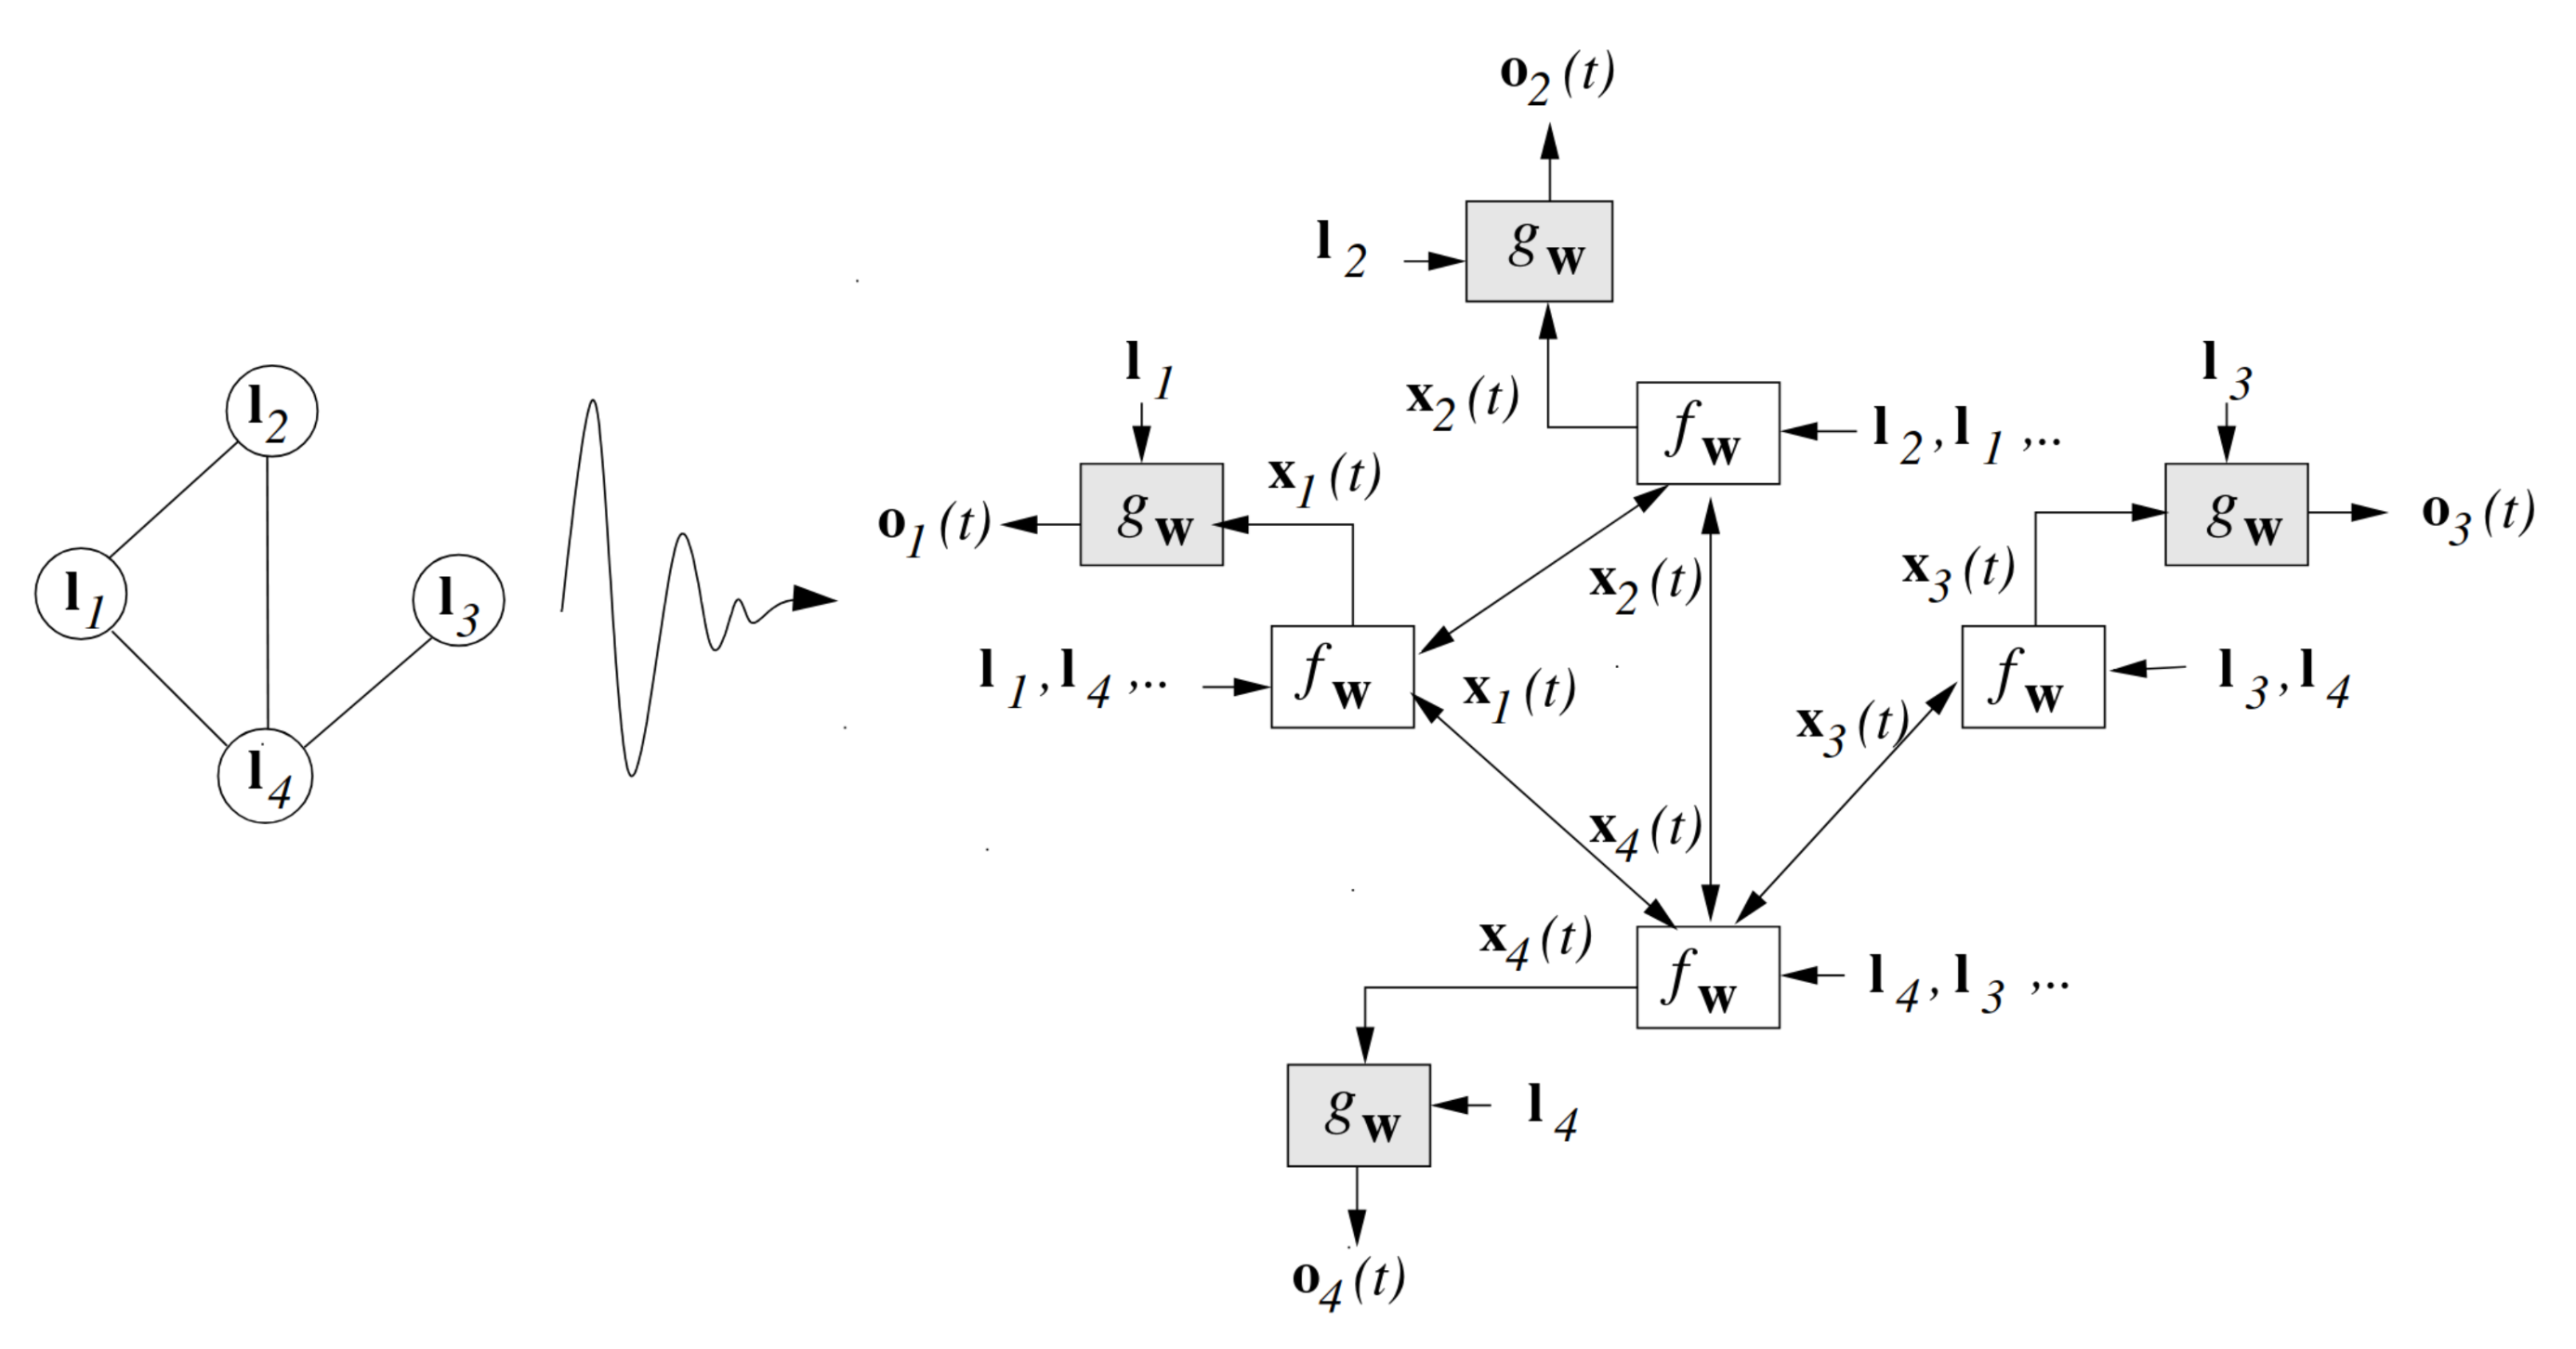
\includegraphics[width=\linewidth]{images/GNN-gori.png}
	\caption{A simple graph with 4 nodes and the corresponding graph neural network. Original figure from \cite{gori_new_2005}. Different notation used, with \( \mathvec{x} \) denoting the hidden state and \( \mathvec{l} \) denoting a node label.}
	\label{fig:gori}
\end{figure}

\section{Random Walk-Based and Convolutional Models for Graph Machine Learning}

Graph machine learning models can be broadly categorized into two main types: random walk-based models and convolutional models.

Random walk-based models utilize random walks to explore the structure of a graph. These models, such as DeepWalk and node2vec, generate sequences of nodes by simulating random paths through the graph. By analyzing these sequences, the models capture the local neighborhood structure and learn low-dimensional embeddings that reflect the relationships between nodes.

Convolutional models, on the other hand, extend the concept of convolution from traditional grid-like data (such as images) to graph data, allowing them to directly leverage the graph structure. Examples of these models include Graph Convolutional Networks (GCNs), Graph Attention Networks (GATs), and GraphSAGE\@. Convolutional models aggregate information from a node’s neighbors to learn representations that capture both local and global graph structure. By stacking multiple convolutional layers, these models can learn increasingly complex patterns and interactions in the graph data, enabling them to make predictions based on the node features and their connections.

Both types of models exploit the graph's topology in different ways to learn meaningful representations of nodes, edges, and the overall graph, allowing for effective predictions and analysis in a variety of applications.

\subsection{Random Walk-Based Models}

Random walk-based models utilize random walks to explore the structure of a graph and understand the relationships between its nodes. A random walk is a process that starts at a given node and moves to a neighboring node at random, continuing this process for a specified number of steps. These walks effectively sample the graph, providing a means to understand the local and, to some extent, global structure of the graph without needing to process the entire graph at once. The following models are, however, all transductive and need to have the whole graph available during training. Due to this, the models can't generalize to samples which were not present during training, as those wouldn't be contained in any of the random walks.

\subsubsection{DeepWalk}

\name{DeepWalk} is one of the pioneering random walk-based methods for learning node embeddings. It treats random walks as equivalent to sentences in natural language processing and applies the Skip-gram model to learn embeddings. See Figure~\ref{fig:deepwalk-motivation} for a motivating example of the similar distributions of word occurrences and vertex occurences in random sequences.

\begin{figure}
	\begin{subfigure}{0.49\linewidth}
		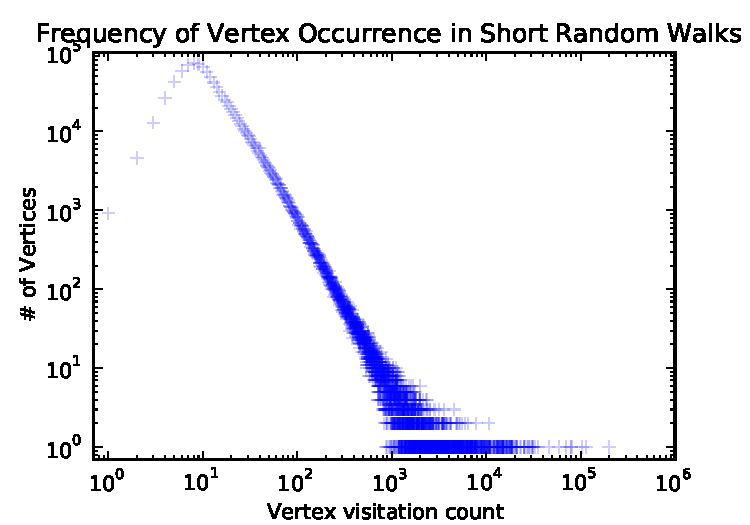
\includegraphics[width=\linewidth]{images/deepwalk-motivation/youtube-powerlaw.pdf}
	\end{subfigure}
	\begin{subfigure}{0.49\linewidth}
		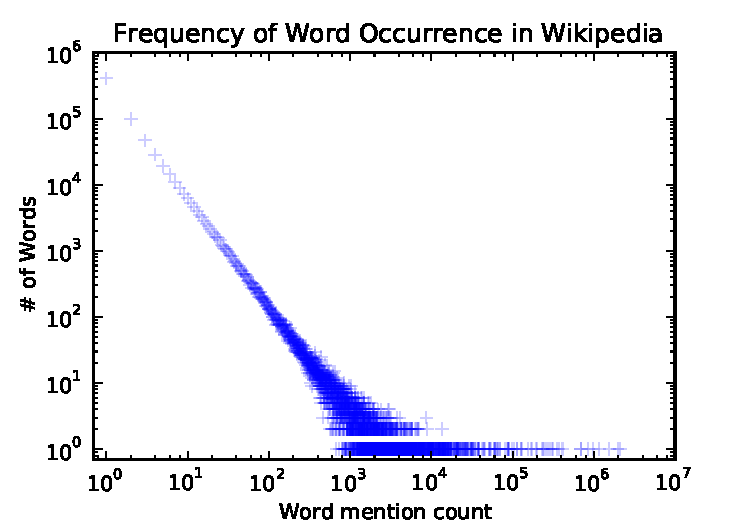
\includegraphics[width=\linewidth]{images/deepwalk-motivation/wiki-powerlaw.pdf}
	\end{subfigure}
	\caption{The distribution of vertices appearing in short random walks follows a power-law, much like the distribution of words in natural language. Original figure from \cite{perozzi_deepwalk_2014}.}
	\label{fig:deepwalk-motivation}
\end{figure}

The DeepWalk algorithm generally consists of two steps -- the generation of random walks from a graph and the extraction of node embeddings from these random walks. The first step is fairly straightforward, the algorithm chooses a random node \( v_i \in V \) as the starting point of the random walk \( \mathcal{W}_{v_i} \) and then constructs the random walk one node at a time by sampling uniformly from the neighbours of the last visited node. This process continues until a desired maximum length \( t \) is reached. In practice, this length is constant across all the random walks generated.

Once a sufficient number of random walks has been generated, these can be used to obtain the node embedding \( \Phi : V \to \mathfield{R}^{\left\lvert V \right\rvert \times d} \). Intuitively, this embedding should maximize the likelihood of observing a given node given all the preceding nodes in the random walk, that is for a random walk \( \mathcal{W} = \left( v_1, v_2, \dots, v_t \right) \), it would maximize
\begin{equation}\label{eq:next-node-probability}
	P \left( v_i \middle| \left( \Phi \left( v_1 \right), \Phi \left( v_2 \right), \dots, \Phi \left( v_{i-1} \right) \right) \right), \quad v_i \in \mathcal{W}
\end{equation}
Computing this objective function, however, quickly becomes unfeasible. Instead, the \name{Skip-gram} algorithm by \cite{mikolov_efficient_2013} is employed. This algorithm, which is visualized in Figure~\ref{fig:skip-gram}, turns the prediction problem on its head by maximizing the probability of preceding nodes in the random walk from the embedding of the current node, instead of Equation~\ref{eq:next-node-probability}. Secondly, instead of only considering the preceding nodes, the algorithm also considers the following nodes. Finally, the order of the nodes in the sequence is disregarded. Together, this gives us the following maximization objective:
\begin{equation}\label{eq:deepwalk-objective}
	P \left( \left\{ v_1, v_2 , \dots, v_{i-1}, v_{i+1}, \dots, v_t \right\} \middle| \Phi \left( v_i \right) \right), \quad v_i \in \mathcal{W}
\end{equation}

\begin{figure}
	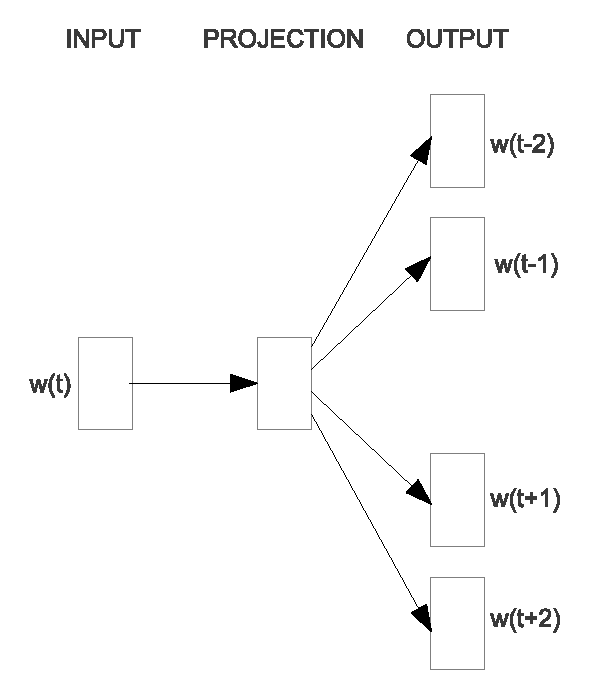
\includegraphics[width=0.6\linewidth]{images/skip-gram.pdf}
	\caption{A schematic representation of the skip-gram algorithm. The embedding (projection) of a word at position \( t \) should maximize the likelihood of surrounding words in the sequence. Original figure from \cite{mikolov_efficient_2013}.}
	\label{fig:skip-gram}
\end{figure}

The algorithm realizes the embedding \( \Phi \) as a matrix of individual node embeddings that is randomly initialized and optimized iteratively over all of the random walks. This optimization is realized as a gradient descent with the objective function being the negative log likelihood of the objective introduced in Equation~\ref{deepwalk-objective}. Further computational optimizations are needed such as a hierarchical softmax algorithm for efficient computation of the node occurence probabilities, however, further details are outside the scope of this work.

\subsubsection{Node2Vec}
